\problemname{Attack on Alpha-Zet}

\begin{wrapfigure}{r}{.3\textwidth}
  \vspace{-5mm}
  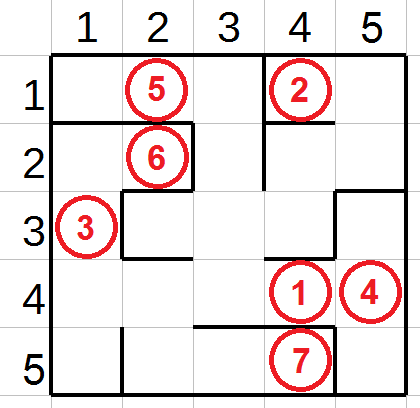
\includegraphics[width=.3\textwidth]{Mazerunner.png}
  \vspace{-1cm}
  \caption{Illustration of Sample Input 2}
\end{wrapfigure}

Space pirate Captain Krys has recently acquired a map of the artificial and highly secure
planet Alpha-Zet which he has been planning to raid for ages. 
It turns out the whole planet is built on a 2D plane with modules that
serve as one room each. There is exactly one module at every pair of integer coordinates and modules are
exactly $1\times1$ units big. Every module is bidirectionally connected to at least one adjacent
module. Also, for any two modules there exists exactly one path between them. All in all the modules 
create a rectangular maze without any loops.

On the map Captain Krys has marked several modules he wants to visit in exactly the
marked order. What he intends to do there is none of your business, but he promises you a
fortune if you determine the number of modules he has to walk through along the
route (since there are no loops he will always take the direct route from one marked
module to the next). The first marked module indicates where he starts his journey, the last
where he wants to finish.

\section*{Input}

The input consists of:
\begin{itemize}
  \item one line with two integers $h$ and $w$ ($2 \le h, w \le 1\,000$) describing the height and
  the width of the maze.
  \item $h+1$ lines follow, describing the maze in ASCII, each line containing $2\cdot w+1$
  characters. The description always follows these rules:
  \begin{itemize}
    \item In every row, columns with odd index (starting at index $1$) contain either vertical walls or
    spaces and columns with even index contain either horizontal walls or spaces.
    \item The first row describes the northern wall of the maze (which always consists only of horizontal
    walls). Every subsequent row describes a row of modules.
    \item A module is located at every even column index. Its western and eastern walls are located 
    at the directly neighboring odd column indices respectively, its northern wall is located at the same 
    column index but one row above and its southern wall can be found at its own position. If a wall 
    is missing, the corresponding position contains a space instead.
  \end{itemize}
  \item After the description of the maze, an integer $m$ ($2 \le m \le 10^4$) is given.
  \item Each of the following $m$ lines describes a marked module with two integer
  coordinates $x$ and $y$ ($1 \le x \le h$; $1 \le y \le w$). The first pair of coordinates is the start
  point of the journey, the last pair the end point. Modules may appear multiple times
  but never twice or more in a row. $(1,1)$ is the top left module and $(h,w)$ is the bottom right module.
\end{itemize}

It is guaranteed that the maze itself is enclosed. Furthermore it is guaranteed that exactly one 
path exists between any two modules.

\section*{Output}

Output one integer, the number of modules Captain Krys has to travel
through if he follows the route in the exact order given in the input.
